% Plan:
%
% Spis treści
% Spis rysunków
% Słowniczek skrótów
%
% Wstęp (1-2 strony): geneza, obszar, zawartość, dokonania autorów, opis struktury pracy
%
% Rozdziały merytoryczne (4-5, zrównoważone objętościowo):
%   Preambuła (ok. 0.5 strony)
%   Punkty merytoryczne (4-6)
%   Podsumowanie rozdziału
%
%   * opis technologii i uzasadnienie wyboru do rozwiązania problemu
%   * analiza wymagań + projekt systemu (architektura)
%   * opis implementacji, sposób uruchomienia
%   * badania eksperymentalne (tutaj także: profiling, opóźnienia)
%
% Podsumowanie pracy / Zakończenie
%   Wnioski końcowe
%   Co się udało / nie udało (+dlaczego!)
%   Możliwości rozwoju
%
% Spis literatury (numerowany, w tekście _muszą_ być odniesienia, ~20 pozycji)
%
%
% INNE:
%   * całość - ok. 60-70 stron
%   * numeracja - nie więcej, niż 3-poziomowa


\documentclass[11pt]{book}
\usepackage[top=3cm, bottom=4cm]{geometry}
\usepackage[usenames,dvipsnames]{color}


% \usepackage[polish]{babel}
\usepackage[utf8]{inputenc}
\usepackage[T1]{fontenc}
\usepackage{fullpage}
\usepackage[pdfborder={0 0 0}]{hyperref}
\usepackage{float}
\usepackage{graphicx}
\usepackage{scrtime}
\usepackage{tabularx}
\usepackage{listings} 
\usepackage{caption}
\usepackage{color}
% \usepackage[toc,acronym]{glossaries}

\newcommand{\code}[1]{\begin{tt}{#1}\end{tt}}

\newcommand{\reqlabel}[1]{{\textcolor{Red}{\textbf{#1}}\label{#1}}}
\newcommand{\reqref}[1]{\hyperref[#1]{{\textcolor{Red}{\textbf{#1}}}}}

\newcommand{\tasklabel}[1]{{\textcolor{Blue}{\textbf{#1}}\label{#1}}}
\newcommand{\taskref}[1]{\hyperref[#1]{{\textcolor{Blue}{\textbf{#1}}}}}


\title{Component-based system for management of multilevel virtualization of networking resources}
\author{Robert Boczek \and Dawid Ciepliński}

\begin{document}

  \maketitle
    
  \tableofcontents

  \chapter*{Division of labour} %podzial pracy
	

  \chapter{Introduction}

    % QoS, rezerwacja zasobów, izolacja we współczesnych systemach informatycznych


  \chapter{Context}  % TODO ładniej

    \section*{Chapter overview}


    \section{QoS-aware networking}


    \section{Resource virtualization approaches}


    \section{Multilevel network virtualization}

      \subsection{Virtual network resources}

      \subsection{Fine-grained QoS control}

      \subsection{Virtual appliances}

      \subsection{,,Network in a box'' concept}


    \section{Applications and benefits of virtual infrastructures}

      \subsection{Testing and simulations}

      \subsection{Improving server-side infrastructure scalability}

      \subsection{Infrastructure as a service}

      \subsection{The role of resource virtualization in the SOA stack}


    \section*{Summary}


  \chapter{Requirements analysis}
    
    \section*{Chapter overview}

    \section{Functional requirements}

      \subsection{Instantiation}

      \subsection{Discovery}

      \subsection{Accounting}  % kz: raczej Monitoring


    \section{Non-functional requirements}

    \section{Underlying environment characteristics}

    \section{General approach and problems it imposes}

      \subsection{Load balancing / Deployment}

      \subsection{Infrastructure isolation}

      \subsection{Broadcast domain preservation}

      \subsection{Constraints}


    \section*{Summary}


  \chapter{Solaris OS as a resource virtualization environment}

    \section*{Chapter overview}

    \section{General information}

    \section{Lightweight OS-level virtualization with Solaris Containers}

    \section{Crossbow - network virtualization technology}

        One of the most important condition in terms of network virtualization is that network traffic should be insulated between virtual machines.
        This kind of isolation can be achieved by having a dedicated physical NIC, network cable and port from the switch to the virtual machine itself. 
        Moreover, switch must also ensure sustainability on every port. In every other case virtual machines will definately interfere between each other.
        In a particular case when we have to share physical NIC between virtual machines the most promising solution is to virtualize NIC hardware and the
         second layer of the OSI/ISO stack where sharing is fair and interferences will be avoided. These approach was adapted in the Crossbow architecture
         in OpenSolaris OS.
        Traffic separation is achieved by fundamental blocks of new architecture which are Virtual NICs (VNICs) created by dividing NIC into many VNICs. 
        A VNIC can be created over NIC or Etherstub ( more about them later ) and be dynamically controlled by the bandwidth and CPU resources assigned to
        it.
        The crossbow architecture has introduced fully paralized network stack structure. Each stack could be seen as fully independent lane (without
        any shared locks, queues, and CPUs) therefore network isolation is guaranteed. Key concept is hardware classification performed by the NIC over 
        which VNIC was created. Each lane has a dedicated buffer for Transmit (Tx) and Receive (Rx) ring. In case when load exceeds assigned limit packets
         must be dropped as it is wiser to dop them then to expend OS CPU resources. 

	\begin{figure}[H]
		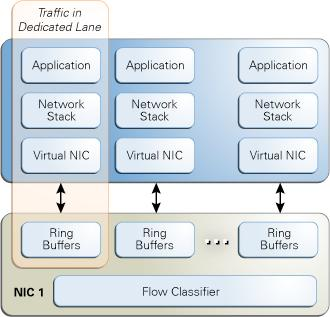
\includegraphics[width=\textwidth]{img/crossbow-traffic-line.jpg}
		\caption{Dedicated lines in the Crossbow architecture}
	\end{figure}

        A virtualization lane can be one of two types, hardware-based or software-based.
        @todo dopisac Hardware-based virtualization lanes i Software-based virtualization lanes


        @todo opisac szczegoly VNIC'ow

        @todo opisac Dynamic Polling and Packet Scheduling

        @todo opisac bandwidth partitioning

        Etherstubs

        As it was mentioned above, the MAC layer provides the virtual switching capabilities which allow VNICs to be created over existing physical NICs.
        In some cases, creating virtual networks without the use of a physical NIC is more welcomed than creating over physical NICs. In that case VNICs 
        would be defined on the top of pseudo NICs. The Crossbow provides these kind of elements which are called Etherstubs. These components could be used
        instead of NICs during creation of VNICs.

        @todo examples of creating vnic and etherstubs
        \textbf{dladm} is the admin command for managing NICs, VNICs and Etherstubs. Below we present a few examples of creating VNICs, Etherstbus and how
        to assigned bandwidth and priority to theses elements.

        \begin{enumerate}
        	\item{dladm create-vnic vnic1 -l e1000g0 - creates new VNIC \textbf{vnic1} over existing NIC \textbf{e1000g0}}
        	\item{dladm create-etherstub ether00 - creates new Etherstub \textbf{ether00}}
        	\item{dladm show-linkprop vnic11 - lists all properties assigned to \textbf{vnic11} link}
        	\item{dladm set-linkprop -pmaxbw=1000 vnic11 - assignes 1Mbps bandwith limit to \textbf{vnic11} link}
        	\item{dladm set-linkprop -ppriority=low vnic11 - assignes low priority to \textbf{vnic11} link}
        \end{enumerate}

        Here we have just presented some basic commands. For more examples see \textbf{man dladm}
        

    \section{Resource access control}

    \section*{Summary}


  \chapter{The system architecture}

    \section*{Chapter overview}

      % tutaj tez kilka slow i JIMSie i integracji + co to daje


    \section{High-level design}


    \section{System components and their responsibilities}

      \subsection{Assigner}

      \subsection{Supervisor}

      \subsection{Worker}


    \section{Crossbow resources instrumentation}


    \section{Domain model and data flows}


    \section*{Summary}


  \chapter{Implementation}
    
    \section*{Chapter overview}


    \section{Implementation environment}


    \section{Domain model transformation details}


    \section{Low-level functions access}


    \section{Building and running the platform}


    \section*{Summary}


  \chapter{Case Study}

    \section*{Chapter overview}

    \section{Clustered GlassFish}

      \subsection{Scenario description}

      \subsection{GlassFish cluster integration}


    \section{Multimedia server}

      \subsection{Scenario description}

      \subsection{Resource access requirements}

      \subsection{Providing tunable and scalable virtual infrastructure}


    \section*{Summary}


  \chapter{Summary}

    \section*{Chapter overview}

    \section{Conclusions}

    \section{Achieved goals}

    \section{Further work}


  \begin{thebibliography}{some-label}

    % TODO bibtex
    
    \bibitem[1]{} Crossbow: From Hardware Virtualized NICS To Virtualized Networks, http://conferences.sigcomm.org/sigcomm/2009/workshops/visa/papers/p53.pdf
    \bibitem[2]{} Virtual switching in Solaris, http://hub.opensolaris.org/bin/download/Project+crossbow/Docs/virtualswitch.pdf
    \bibitem[3]{} Oracle Solaris 11 Express Network Virtualization and Network Resource Management, http://www.oracle.com/technetwork/articles/servers-storage-admin/sol11ecrossbow-186794.pdf

  \end{thebibliography}


\end{document}

% vim: et : spelllang=en_us,pl : spell :
